\begin{figure}[htbp]   
    \caption{Impact of Departed Importance on Organizational Outcomes} \label{fig:prs_opened_more_imp}
    \centering
    \begin{minipage}[b]{0.49\textwidth}
        \centering
        \subcaption{By problem involvement}    \label{fig:prs_opened_involved}
        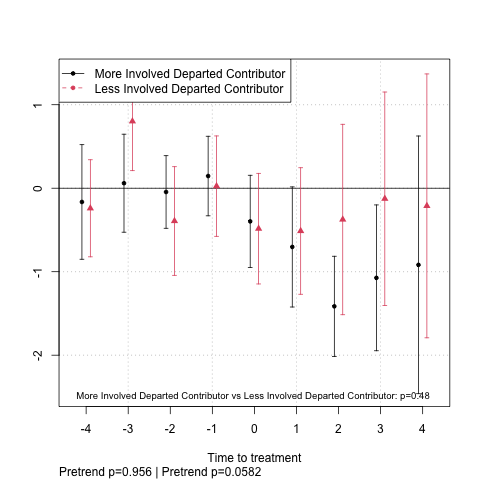
\includegraphics[width=\textwidth]{temp/output/collab/prs_opened_involved_cs_norm.png}
    \end{minipage}
    \begin{minipage}[b]{0.49\textwidth}
        \centering
        \subcaption{By PR opening involvement}    \label{fig:prs_opened_pr_involved}
        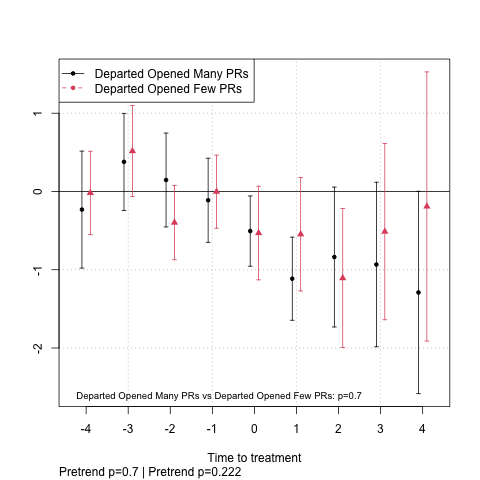
\includegraphics[width=\textwidth]{temp/output/collab/prs_opened_departed_opened_cs_norm.png}
    \end{minipage}
    \begin{minipage}[b]{0.49\textwidth}
        \centering
        \subcaption{More involved}    \label{fig:prs_opened_more_involved}
        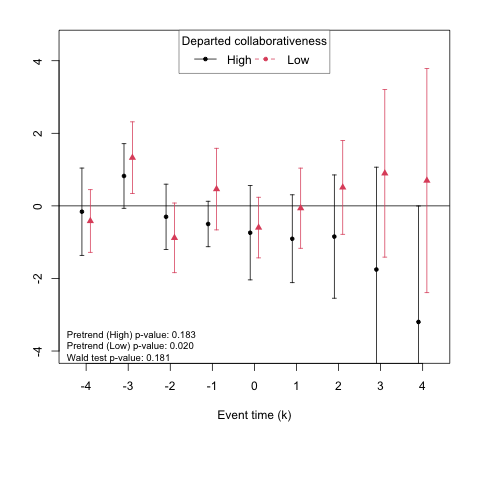
\includegraphics[width=\textwidth]{temp/output/collab_imp/inv0_cs_norm_prs_opened.png}
    \end{minipage}
    \begin{minipage}[b]{0.49\textwidth}
        \centering
        \subcaption{Less involved }    \label{fig:prs_opened_less_involved}
        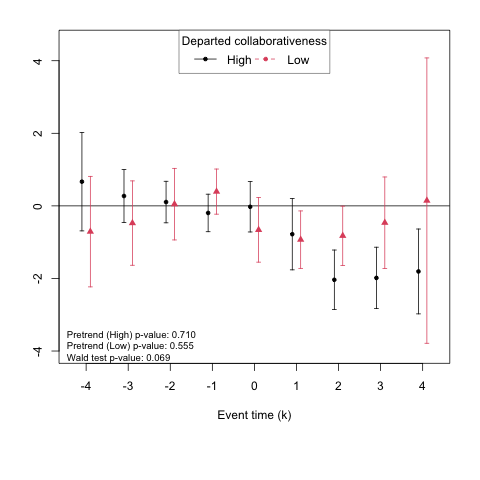
\includegraphics[width=\textwidth]{temp/output/collab_imp/inv1_cs_norm_prs_opened.png}
    \end{minipage}

  \begin{minipage}{1\textwidth}
    \textbf{Figure notes:} 
    Following Callaway and Sant’Anna (2021), I estimate event-study coefficients accompanied by 95\% simultaneous confidence bands. For each plot with event study estimates from two subsamples, I report three Wald-test p-values: one for the pretrend test in the first subsample, one for the pretrend test in the second subsample (both from Equation \ref{eq:wald_test_pretrends} in Section \ref{sec:main_method}), and one for the difference in treatment effects across subsamples (Equation \ref{eq:wald_test} in Section \ref{sec:att_subset}).  Panel~\subref{fig:prs_opened_involved}  subsets organizations by \textbf{departed member involvement}, as defined in Section~\ref{sec:org_level_subset}. Panel~\subref{fig:prs_opened_pr_involved}  subsets organizations by \textbf{departed member pull request involvement}, as defined in Section~\ref{sec:org_level_subset}. Panel~\subref{fig:prs_opened_more_involved} and Panel~\subref{fig:prs_opened_less_involved} condition on organizations where the departed was more and less involved by \textbf{departed member pull request involvement}, respectively and both subset by departed contributor collaborativeness
  \end{minipage}

\end{figure}
